\RequirePackage{plautopatch}
\documentclass[uplatex,dvipdfmx,10pt,a4paper,notitlepage,oneside,twocolumn]{abst_jsarticle}
% notitlepage : \titlepage は独立しない
% oneside : 奇数・偶数ページは同じデザイン
% twocolumn : 2段組
% \setlength{\textwidth}{\fullwidth}
% 本文領域はページ一杯で, 傍注の幅を取らない
\usepackage[dvipdfmx]{graphicx}
\usepackage[dvipdfmx,x11names]{xcolor}
\usepackage{amsmath,amssymb}
% \numberwithin{equation}{section}
\usepackage{url}
\usepackage{bm}
\usepackage[hang, small, bf, labelsep=quad]{caption}

\usepackage{comment}
%%%
\usepackage{here}
\usepackage{algorithm}
\usepackage{algorithmic}
\usepackage{hhline} 
\usepackage[subrefformat=parens]{subcaption}
\captionsetup{compatibility=false}
%%%

\columnsep=10mm
\setlength{\hoffset}{-0.85cm}
\setlength{\voffset}{-2.0cm}
\setlength{\textwidth}{53zw}   %横25字
\setlength{\textheight}{78zw}

% \renewcommand{\baselinestretch}{0.8}
%upTex(ptex2pdf)
\usepackage{fancyhdr}
\fancypagestyle{firstpage}
{
   \fancyhead[L]{中央大学大学院理工学研究科2024年度修士論文}
   \fancyhead[R]{}
   \fancyfoot{}
   \renewcommand{\headrulewidth}{0pt}
}

\title{
\textbf{\textgt{煙シミュレーションのための部分空間法の高速化}}\\
%\vspace*{0.3cm}
\textsf{Accelerated Subspace Method for 3D Smoke Simulation}\\
}
\author{
{\large \textbf{\textgt{情報工学専攻 須之内 俊樹}}}\\
{\large \textsf{Toshiki SUNOUCHI}}
}

\date{}
\pagestyle{empty}

\begin{document}

\maketitle
%%%%%%%%%%%%%%%%%%%%%%%%%%%%%%
\thispagestyle{firstpage}

\begin{abstract}
流体シミュレーションに部分空間法を適用することで,各時刻のシミュレーションを大幅に高速化することができるが,前処理に膨大な計算時間がかかることが課題である.
そこで本研究は,前処理をシミュレーション時間に対して分割し,前処理全体の計算時間を削減する手法を提案する.計算機実験の結果,前処理のボトルネックとなっている基底計算のための特異値分解の高速化を確認し,前処理の高速化に有効であると示すことができた.また,計算結果の精度について,基底の累積寄与率や相対誤差を用いて評価をし,分割数によるシミュレーションのレンダリング結果の変化を確認した.
\end{abstract}


\vspace{1zw} \noindent
\textbf{\textgt{キーワード:}} 
流体シミュレーション,部分空間法,スナップショット固有直交分解,立体求積法.


\section{はじめに} \label{sec:section1}

流体シミュレーションは,工学およびコンピュータグラフィックスの分野において広く利用されている.コンピュータグラフィックスの分野では,現実的な水や煙のアニメーションを生成し,映像作品やゲームの演出に活用されている.コンピュータグラフィックスにおいては,物理的に厳密なシミュレーションよりも,視覚的に自然な動きを高速に計算することが求められる.

近年,より高解像度の流体シミュレーションが求められる中で,計算負荷の増大が課題となっている.そのため,高速化手法の研究が活発に進められており,特に大規模並列計算技術の適用が重要視されている.多くの高速化手法がGPU上での実装を前提として検討されている.

計算負荷の削減手法の一つとして,前処理によりシミュレーション計算に使用する行列の次元を削減する部分空間法が存在する.部分空間法を適用することで,シミュレーション計算そのものは高速化されるが,前処理に要する計算負荷やメモリ使用量が大きくなるという課題がある.
本研究では,部分空間法の計算負荷を削減することにより,前処理に要する時間の短縮を目的とする.

\section{関連研究}
\subsection{煙の流体シミュレーション}
下記の式\ref{eq:Navie}で表される式を,ナビエ・ストークス方程式とよび,これは流体力学の支配方程式である.式 \ref{eq:Navie}の右辺の第一項を移流項,第二項を圧力項,第三項を粘性項,第四項を外力項と呼ぶ.コンピュータグラフィックスにおける気体の外力には重力のほか,温度差による対流を発生させる力や.気体の渦運動を生成する力などが含まれ,これらを適用することで,気体の自然な挙動を再現することが可能となる.式\ref{eq:uncompressed} は流体の非圧縮性条件であり,煙のシミュレーションにおいて流速が著しく大きい場合を除き,利用することが可能である.
	\begin{equation}\label{eq:Navie}
		\frac{\partial}{\partial t}\bm{u} (t)  = - (\bm{u} (t)  \boldsymbol{\cdot}\nabla) \bm{u} (t)   - \frac{1}{\rho}\nabla \bm{p} (t)  + \nu\nabla^2\bm{u} (t)  + \bm{f}
	\end{equation}
	
	\begin{equation}\label{eq:uncompressed}
		\nabla\boldsymbol{\cdot}\bm{u} (t)  = 0
	\end{equation}
	
コンピュータグラフィックスにおいては,ナビエ・ストークス方程式の数値解法の中でも,全ての項を個別に分割して解く手法としてフラクショナルステップ法 \cite{Chorin}が一般的に用いられている.フラクショナルステップ法は,中間子$\bm{u_0}$から$\bm{u_3}$を用いて,ナビエ・ストークス方程式を以下のように分割する.
\[
	\bm{u_0} =  \bm{u} (t)  - \varDelta t \bm{f} 	
\]
\[
	\bm{u_1}(\bm{x}) = \bm{u_0}(\bm{x}  - \varDelta t \bm{u_0})
\]
\[
	\bm{u_2}   =  \bm{V}\bm{u_1}
\]
\[
	\bm{b} = \bm{W}\bm{u_2}
\]
\[
	\bm{p} = \bm{A^{-1}}\bm{b}
\]
\[
	\bm{u} (t+1) = \bm{u_3}  =  \bm{u_2} - \bm{Y}\bm{p} 
\]
ここで,$\bm{V}$,$\bm{A}$は離散ラプラシアン行列を用いて$\nabla^2$を離散化し,それぞれ定数の係数を乗算したものであり,$\bm{W}$,$\bm{Y}$は勾配演算子$\nabla$を離散化したものである.
流速に従って煙の密度を計算し,ボリュームレンダリングによって可視化することで,煙のアニメーションを作成できる.ボリュームデータを三次元的な広がりの様子を把握できるようにレンダリングする手法をボリュームレンダリングという.描画対象の表面のみをレンダリングするサーフェスレンダリングとは異なり,光の散乱や吸収などの光学的性質を利用して,描画対象の内側のデータも出力画像に反映させる.
\subsection{部分空間法}
部分空間法は,ベクトル空間をより低次元の部分空間に射影し,数値シミュレーションにおける計算負荷を軽減する手法である.流体シミュレーションにおける部分空間法は,モデル縮約やモデル縮退とも呼ばれている.扱うベクトルデータやシミュレーションの計算を低次元の部分空間に射影して行い計算負荷を軽減する.

まず,線形項の計算手法\cite{projection_base}について説明する.シミュレーションの前処理として,$n$次元ベクトル$\bm{x}$を$r$次元ベクトル$\bm{\widetilde{x}} $に変換する,$n \times r$直交行列$\bm{A}$を考える.直交行列の性質から,以下の2式が成り立つ.
 	\begin{align*}
 		\bm{\widetilde{x}}  		&= \bm{A^{\mathsf T}}\bm{x}		&\bm{x} 			&= \bm{A}\bm{\widetilde{x}}
	\end{align*}
	また,$\bm{\widetilde{x'}}  = \bm{A^{\mathsf T}}\bm{x'}$を満たす$n$次元ベクトル$\bm{x'}$,$r$次元ベクトル$\bm{\widetilde{x'}} $について,以下の2式が成り立つような,任意の$m \times n$行列$\bm{F}$,任意の$m \times r$行列$\bm{\widetilde{F}}$を考える.
	 \begin{align*}
		\bm{x'} 			&= \bm{F}\bm{x}		&\bm{\widetilde{x'}} 		&= \bm{\widetilde{F}}\bm{\widetilde{x}} 
	\end{align*}
	以上の4式を用いて,行列$\bm{F}$と$\bm{\widetilde{F}}$の間の以下の関係式が得られる.
	\[
	\bm{\widetilde{F}} = \bm{A^{\mathsf T}}\bm{F}\bm{A}
	\]

次に,非線形項について説明する.
非線形項については,立体求積法(Cubature Method)を用いた積分計算の計算量削減手法\cite{subspace}を用いて次元削減を行う.非線形関数$\mathcal{F}$について,$\bm{f} = \mathcal{F}(\bm{x})$とする.ここで,$\bm{f}$,$(\bm{x})$は$n$次元ベクトルである.削減前の$\bm{f}$は,$\mathcal{F}$をシミュレーション空間$\Omega$の全ての計算点$\bm{x_p}$において積分することで求められる.
\[
	\bm{f} = \int_\Omega\mathcal{F}_p(\bm{x_p})
\]
この積分計算を立体求積法を用いて次元削減する.
立体求積法はシミュレーション空間全域から適切に計算点を有限個サンプリングし,重み付き和をとることで積分計算を離散化する.
サンプリングした点集合を$P$,サンプリング点$p$に対応する重みを$w_p$とすると,立体求積法は以下のように表せる.
\[
	\bm{f} = \sum_{p=1}^Pw_p\mathcal{F}_p(\bm{x_p})
\]
この式は速度に関する基底を用いて以下のように部分空間へ射影することが可能である.
\[
	\bm{U_1}\bm{f} = \sum_{p=1}^Pw_p(\bm{U^p})^{\mathsf T}\mathcal{F}_p(\bm{U^p}\bm{x})
\]

適切なサンプリング点の集合と重みの計算にかかる計算量は,文献\cite{subspace}のNNLS(Non Negative Linear Solve)ソルバによる手法を用いると$O(P\times rTP^2) = O(rTP^3)$である.
\section{スナップショット分割による高速化}
\subsection{フラクショナルステップ法への部分空間法の適用}
フラクショナルステップ法では,中間子$\bm{u_0}$から$\bm{u_3}$までの4種類の速度ベクトルを計算する.それぞれの速度ベクトルを部分空間に射影するため,対応したスナップショット行列が1つずつ必要である.中間子$\bm{u_i}$から得た基底を$\bm{U_i}$,$\bm{p}$から得られた基底を$\bm{P}$とする.
フラクショナルステップ法の線形項の計算を部分空間に射影すると,以下のようになる.
\begin{align*}
 \bm{U_2^{\mathsf T}}\bm{u_2}	& = (\bm{U_2^{\mathsf T}}\bm{V}\bm{U_1})\bm{U_1^{\mathsf T}}\bm{u_1} 					&\bm{\widetilde{u_2}} 		&= \bm{\widetilde{V}}\bm{\widetilde{u_1}}	\\
 \bm{P^{\mathsf T}}\bm{b}		& = (\bm{P^{\mathsf T}}\bm{W}\bm{U_2})\bm{U_2^{\mathsf T}}\bm{u_2}        				&\bm{\widetilde{b}}			&= \bm{\widetilde{W}}\bm{\widetilde{u_2}}	\\
 \bm{P^{\mathsf T}}\bm{p} 		&= (\bm{P^{\mathsf T}}\bm{A}^{-1}\bm{P})\bm{P^{\mathsf T}}\bm{b}						&\bm{\widetilde{p}}			&= \bm{\widetilde{A}}\bm{\widetilde{b}}\\
 \bm{U_3^{\mathsf T}}\bm{u_3} 	&=  \bm{U_2^{\mathsf T}}\bm{u_2} - (\bm{U_3^{\mathsf T}}\bm{Y}\bm{P})\bm{P^{\mathsf T}}\bm{p}	&\bm{\widetilde{u_3}}		&= \bm{\widetilde{u_2}}  -  \bm{\widetilde{Y}}\bm{\widetilde{p}}
\end{align*}

部分空間法によるシミュレーション計算は,前処理として基底と部分空間に射影した行列を計算する.基底を計算するステップの計算量のボトルネックは,QR分解の$O(nm^2)$である.部分空間に射影した行列を計算するステップについては,射影前のそれぞれの行列が非常に疎であるため,基底の計算ほど時間はかからない.

非線形項は立体求積法を用いて計算する.立体求積法に用いる基底は,外力項は$\bm{U}_0$であり,移流項は$\bm{U}_1$である.
例えば,移流項を最終的な部分空間に射影した移流項計算は以下のようになる.
\[
	\bm{\widetilde{u_2}} = \sum_{p=1}^Pw_p\bm{\widetilde{f}}_p =   \sum_{p=1}^Pw_p(\bm{U^p_1})^{\mathsf T}\mathcal{F}_p(\bm{\widetilde{u_1}})
\]
\subsection{部分空間法の高速化手法の提案}
部分空間法の前処理において,基底の計算と行列の射影の計算量はスナップショットの$2$乗に比例し,前処理の大多数の時間を占めている.本節では部分空間法の前処理の高速化を達成するため,スナップショットを$d$個に分割する手法を提案する.

部分空間法の基底の計算に用いるスナップショットを$d$分割することによって,基底1つの計算負荷$O(nm^2)$が$\frac{1}{d^2}$に削減される.アルゴリズム全体では$d$回計算するため,計算負荷は$\frac{1}{d}$になることが期待できる.行列の射影計算も分割した基底ごとに行う.空間計算量のボトルネックは分割前のスナップショット行列であり,分割前と変わらない.しかし,特異値分解する行列のサイズが$\frac{1}{d}$になることで,GPUを用いた大規模高速計算と併用する場合,GPUメモリの削減が期待できる.空間計算量をGPUが一度に扱うことができる値まで削減することで,並列計算による高速化が期待できる一方で,特異値分解の回数が$d$倍になることで,CPU-GPU間のデータ通信の時間が増加することに注意が必要である.

\section{計算機実験}
本研究では,C++と線形代数ライブラリEigenを用いて,文献\cite{fedkiw}の煙の流体シミュレーションを行うソフトウェアを実装した.立方体形状のシミュレーション空間の底面中心から,煙が立ち上る様子をシミュレーションし,そのデータを元に部分空間法による次元削減を行なった.また,OpenGLを用いてスライスベースのボリュームレンダリングを行い,実験結果を可視化するソフトウェアを実装した.これによって得られたシミュレーション結果と,提案手法の計算負荷と削減後のデータの精度について調査を行った.計算負荷の評価は,部分空間法の基底を計算する前処理と行列の射影について実行時間を計測した.データの精度は相対誤差を用いて評価を行なった.ここで相対誤差$L_2$は次元削減前後のベクトル$\bm{u}$と$\bm{\widetilde{u}}$について,以下のように表される.また,基底の精度を累積誤差を用いて評価した.

\[
L_2 = \frac{|| \bm{u} - \bm{\widetilde{u}} ||_2}{||  \bm{u} ||_2}
\]

表\ref{tab:basis}は基底の計算にかかった実行時間,表\ref{tab:projection}は行列の射影にかかった実行時間を解像度と分割数ごとに計測した結果である.基底の計算については分割数が大きくなるほど高速化に成功している.一方で,行列の射影に関しては,低解像度では分割数が大きいほど高速になっているが,高解像度における目立った高速化は見られなかった.

表\ref{tab:ruiseki}は,基底の累積寄与率を解像度と分割数ごとに計測した結果である.分割数が大きい基底の累積寄与率は,最大値最小値ともに大きくなっているのがわかる.

また,図\ref{fig:128error}は,解像度$128^3$における,流速の$L_2$誤差の時間推移を表したグラフである.スナップショットの分割の直後に$L_2$誤差が減少している.また,流れの時間変化が少ないシミュレーションの後半では,分割なしと比べて精度が向上している.図\ref{fig:n128_f99}は,シミュレーション結果のレンダリング画像のうち,誤差が大きく変化した100フレーム目と101フレーム目のもので,上段が元のシミュレーション結果,中段が分割なし,下段が分割数2のものである.また,密度の誤差によって誤差が小さい部分は青く,誤差が大きい部分は赤く色をつけている.流速の誤差に基づいて,煙の密度分布に誤差が発生しているのがわかる.

非線形項については追加の実験を行ったところ,サンプリングされる点によって重みの計算が発散する場合がある.計算時間はスナップショット数については線形時間であるが,サンプリングする点の数が減ることによりNNLSソルバの反復回数が減ることで,実質的に高速化が見込めることもあった.

\begin {table}[htbp]
    \centering
  \caption{基底計算の解像度と分割数ごとの実行時間(秒)}
  \label{tab:basis}
  \begin {tabular}{rrrrr} \hline
    \multicolumn{1}{c}{解像度} 					&\multicolumn{1}{c}{分割なし} 		&\multicolumn{1}{c}{分割数2}			&\multicolumn{1}{c}{分割数4} 		&\multicolumn{1}{c}{分割数10}\\ \hline
    $64^3$ 					& 23.43 			&14.56	 		&8.98	 	&3.78\\
    $128^3$ 				& 190.54 			&118.49 			& 69.62 		&33.43\\ \hline
  \end {tabular}
\end {table}

\begin {table}[htbp]
    \centering
  \caption{行列の射影の解像度と分割数ごとの実行時間(秒)}
  \label{tab:projection}
  \begin {tabular}{rrrrr} \hline
    \multicolumn{1}{c}{解像度} 					&\multicolumn{1}{c}{分割なし} 		&\multicolumn{1}{c}{分割数2}			&\multicolumn{1}{c}{分割数4} 		&\multicolumn{1}{c}{分割数10}\\ \hline
    $64^3$ 					& 3.51 			&2.82	 		&0.85	 		&0.67\\
    $128^3$ 				& 5.21 			& 3.06 			& 3.05 			&3.98\\ \hline
  \end {tabular}
\end {table}

\begin {table}[htbp]
    \centering
  \caption{基底の累積寄与率の最小値と最大値}
  \label{tab:ruiseki}
  \begin {tabular}{rrrrr} \hline
    \multicolumn{1}{c}{解像度} 					&\multicolumn{1}{c}{分割なし} 		&\multicolumn{1}{c}{分割数2}			&\multicolumn{1}{c}{分割数4} 		&\multicolumn{1}{c}{分割数10}\\ \hline
    $64^3$ 									& 0.969886					& 0.972114						&0.979512	 				&0.992557				\\
    										&							&0.985917						&0.990411					&0.996893				\\ \hline
    $128^3$ 								&0.940446 					&0.954735						&0.971454	 				&0.988967				\\ 
    										&							&0.96489							&0.976306					&0.996132				\\	\hline
  \end {tabular}
\end {table}
\begin{figure}[htbp]
\centering
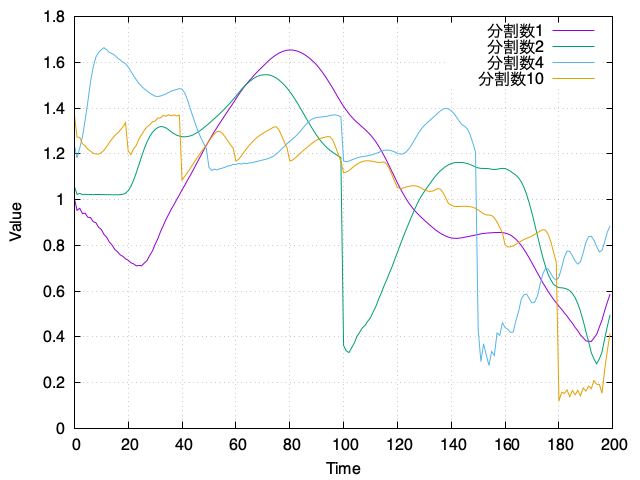
\includegraphics[width=80mm]{images/128error_obstacle.png}
\caption{$解像度128^3における相対誤差$}
\label{fig:128error}
\end{figure}

%\begin{figure}[htbp]
%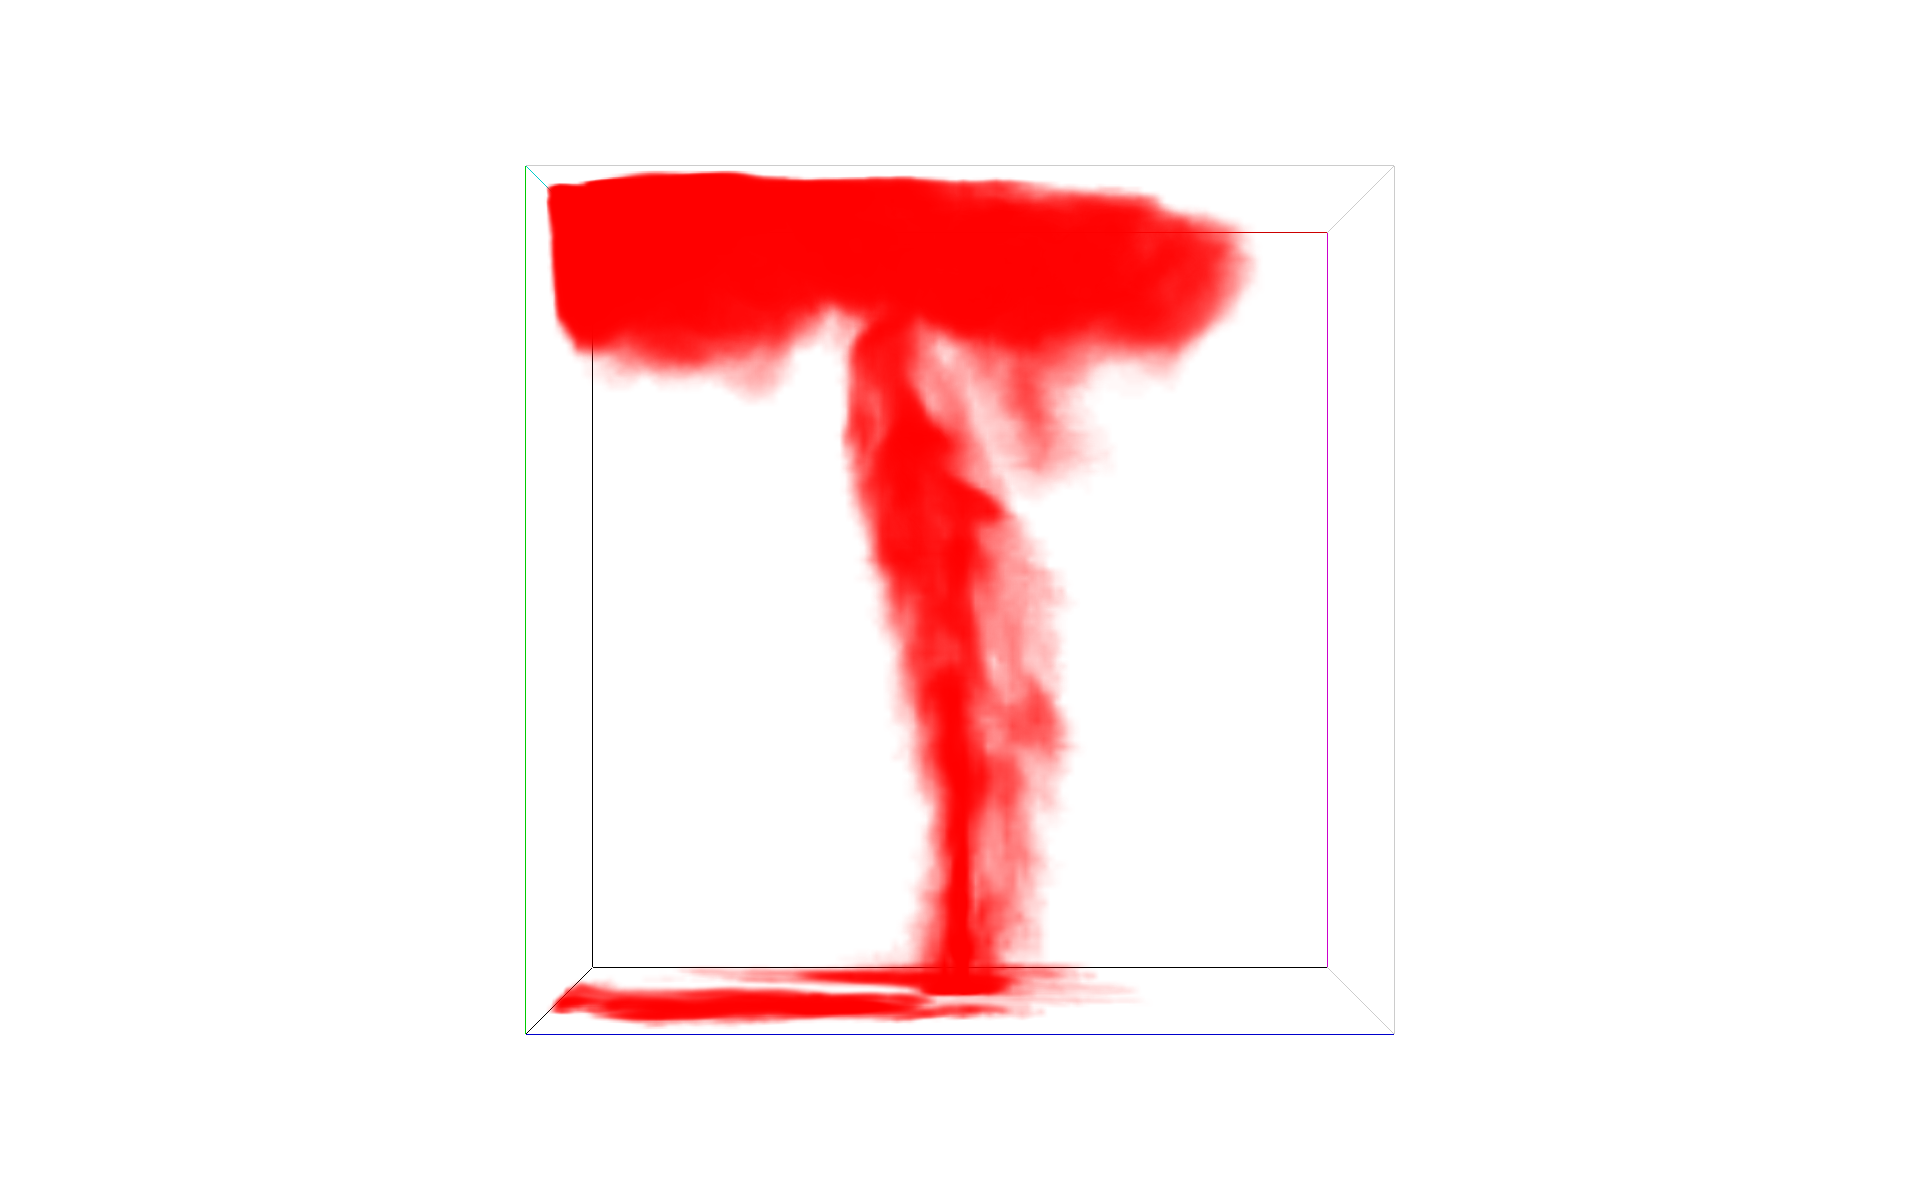
\includegraphics[width=140mm]{images/n128_f99_truth.png}
%\caption{$解像度128^3,ground truth,99フレーム目$}
%\label{fig:n128_f99_div4}
%\end{figure}
%\begin{comment}
\begin{figure}[htbp]
\centering
\caption{$解像度128^3のレンダリング結果$}
\label{fig:n128_f99}
\begin{tabular}{cc}
\begin{minipage}[b]{0.45\linewidth}
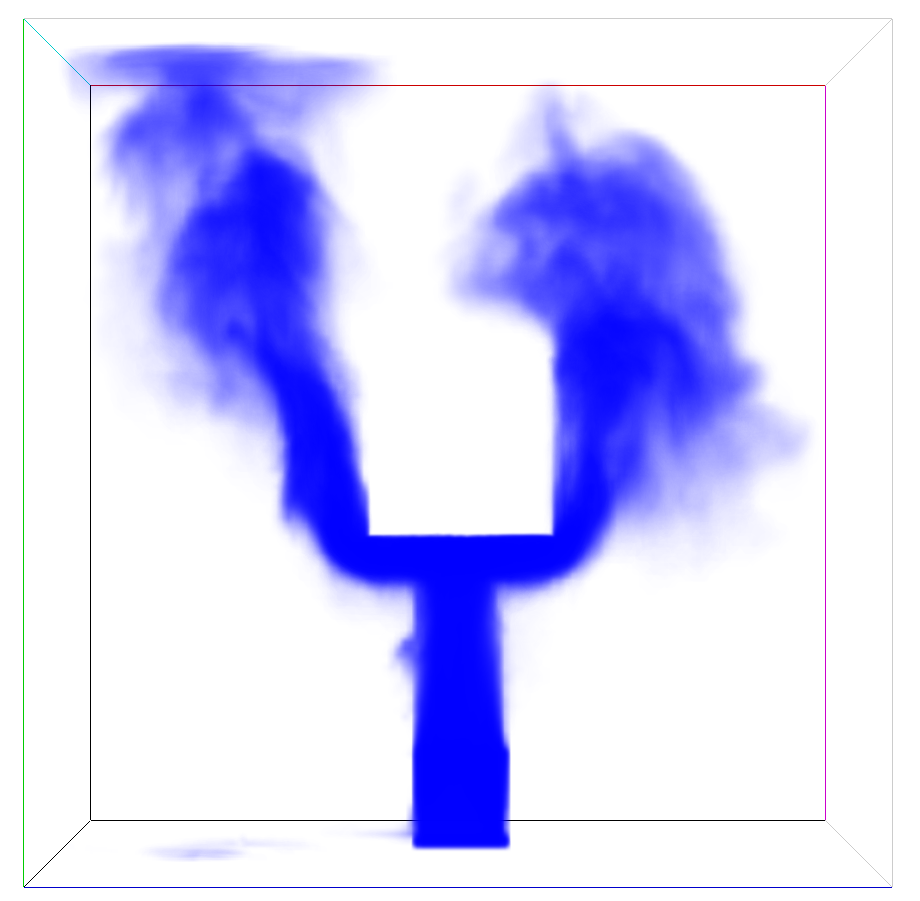
\includegraphics[width=35mm]{images/n128_origin_f99_obstacle.png}
\subcaption{gruound truth 100フレーム目}
\label{fig:ground_truth_99}
\end{minipage}

\begin{minipage}[b]{0.45\linewidth}
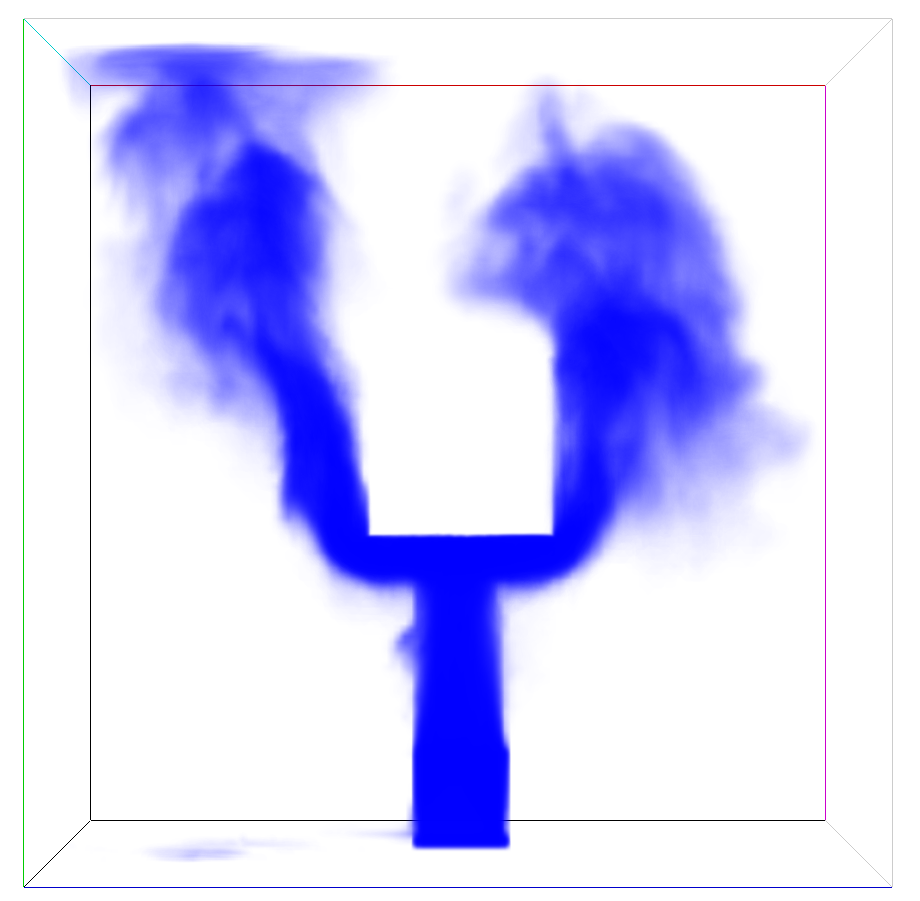
\includegraphics[width=35mm]{images/n128_origin_f100_obstacle.png}
\subcaption{gruound truth 101フレーム目}
\label{fig:ground_truth_99}
\end{minipage}

\\
\begin{minipage}[b]{0.45\linewidth}
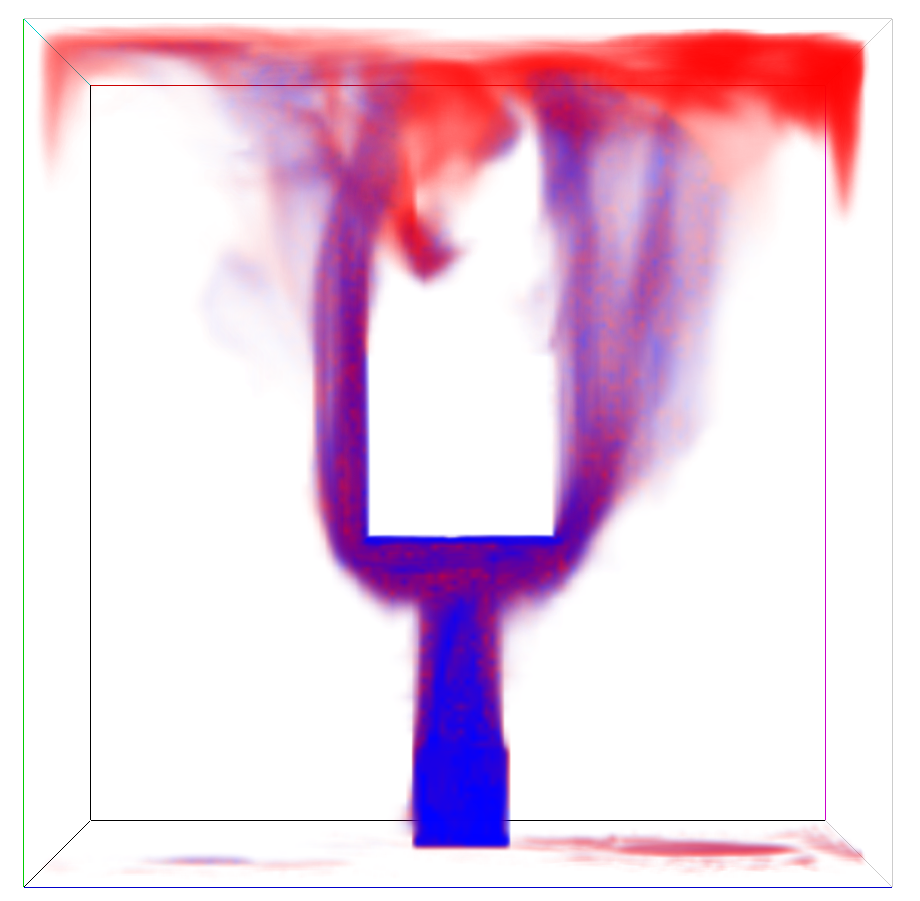
\includegraphics[width=35mm]{images/n128_dev1_f99_obstacle_color.png}
\subcaption{分割数1,100フレーム目}
\label{fig:div1_f100}
\end{minipage}
\begin{minipage}[b]{0.45\linewidth}
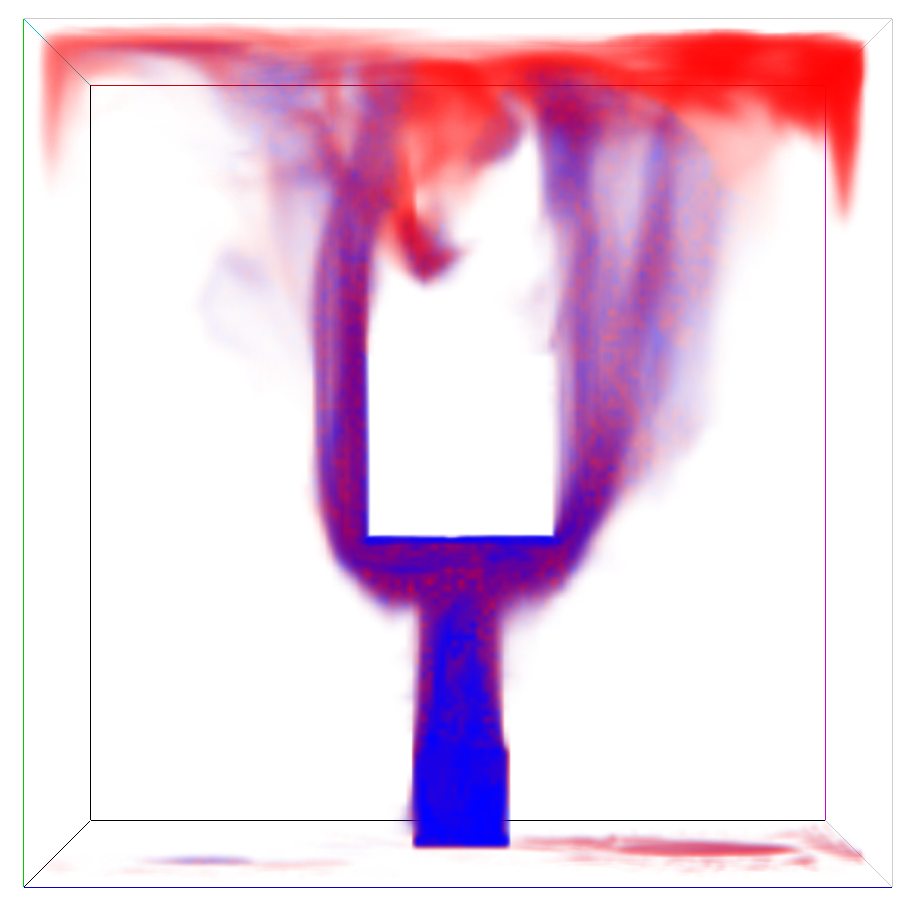
\includegraphics[width=35mm]{images/n128_dev1_f100_obstacle_color.png}
\subcaption{分割数1,101フレーム目}
\label{fig:div1_f100}
\end{minipage}
\\
\begin{minipage}[b]{0.45\linewidth}
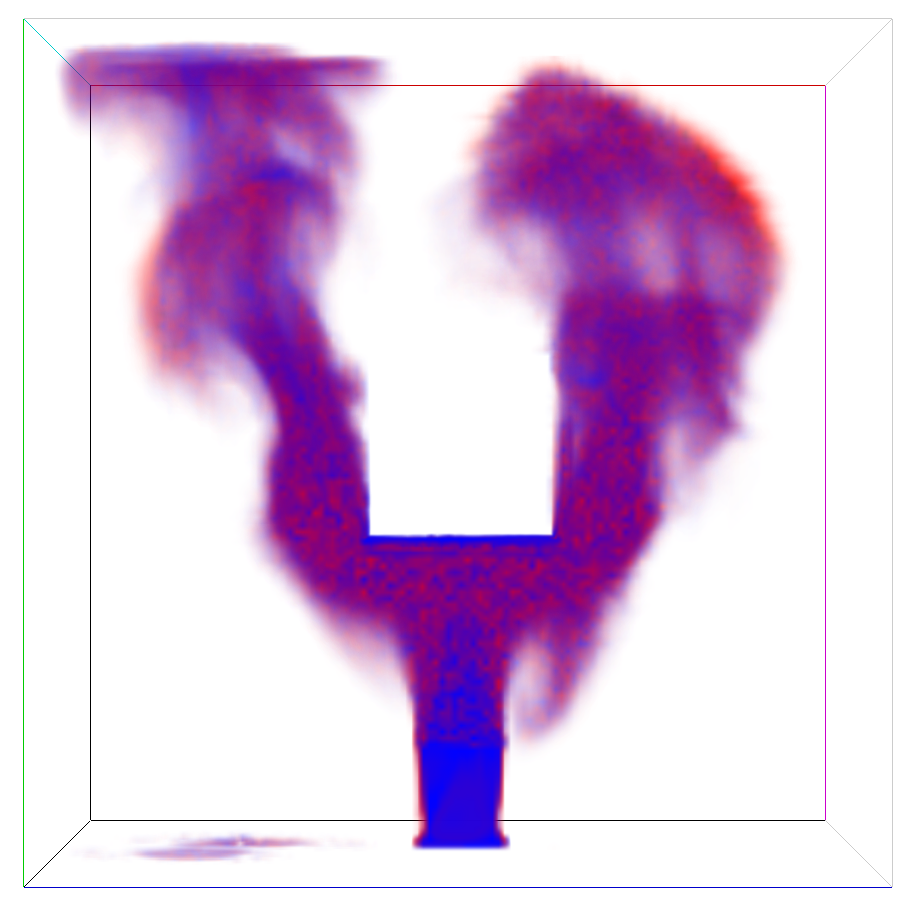
\includegraphics[width=35mm]{images/n128_dev2_f99_obstacle_color.png}
\subcaption{分割数2,100フレーム目}
\label{fig:div2_f99}
\end{minipage}

\begin{minipage}[b]{0.45\linewidth}
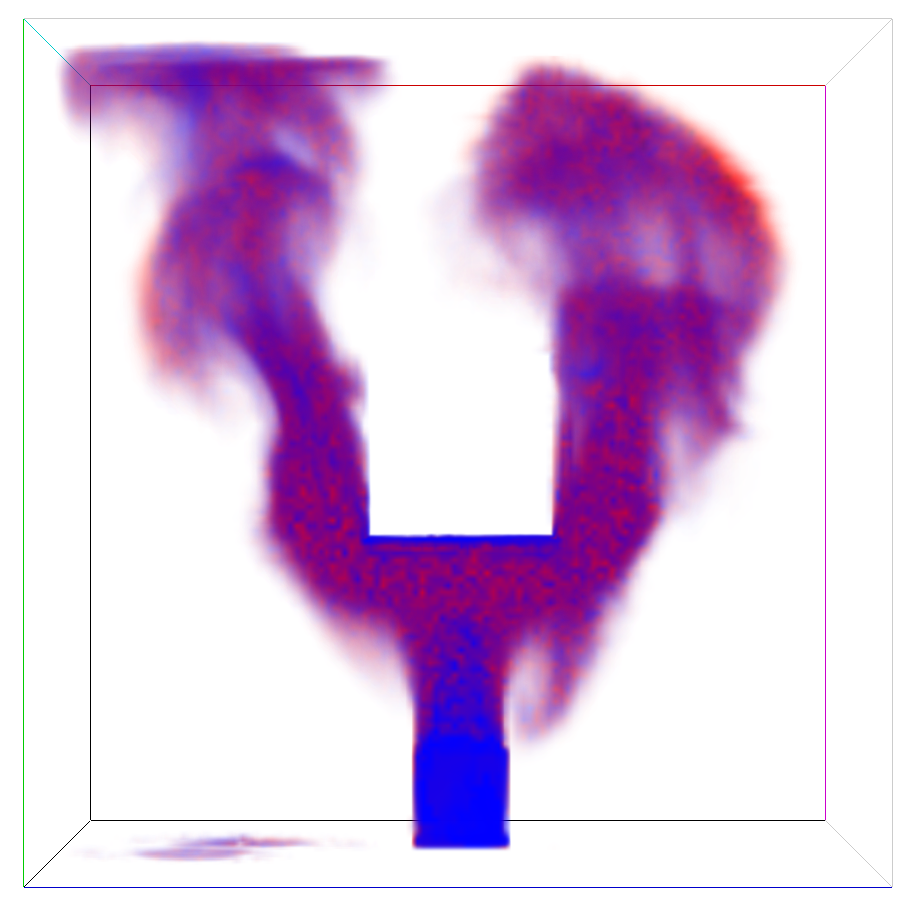
\includegraphics[width=35mm]{images/n128_dev2_f100_obstacle_color.png}
\subcaption{分割数2,101フレーム目}
\label{fig:div2_f100}
\end{minipage}
\end{tabular}
\end{figure}

%\begin{figure}[htbp]
%\centering
%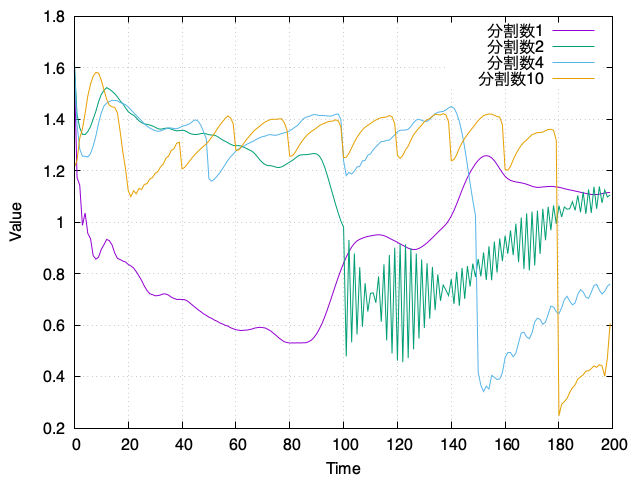
\includegraphics[width=80mm]{images/64error.png}
%\caption{$解像度64^3におけるL_2誤差$}
%\label{fig:64error}
%\end{figure}


%\end{comment}
\section{考察}
部分空間法において,基底による近似誤差が常に発生する.特に急激な流れの変動があった場合,元のデータを十分に近似するには多数のモードを用いる必要があり,用いる基底が固定されていると元の流れを再現できず,誤差が発生する.これに対して,基底を切り替えたとき精度が誤差が大きく減少する.これはスナップショットの範囲を限定した基底を用いることで,流れの特徴をよりよく再現することができたためと考えられる.特に障害物ありのシミュレーションにおいて,障害物との衝突により流れが急速に変化するため,基底を切り替えたことでより良い再現ができたと考えられる.一方で,速度の局所的な精度向上は,密度分布にはすぐに反映されない.これは密度は流速に従って逐次的に変化するためである.

分割後の累積寄与率は分割前よりも大きいのに対して,シミュレーションの相対誤差は分割後の方が大きい場合がある.これは,累積寄与率は直接シミュレーションの誤差を測る指標ではないためである.特に抽出するモードが細部の流れを再現できない場合に誤差が大きくなる可能性がある.

\section{終わりに}
流体シミュレーションにおける部分空間法の前処理にかかる計算時間に対し,スナップショットを分割することによって高速化する手法を提案した.特に基底計算については分割数に応じた高速化を達成し,前処理全体の高速化を達成した.スナップショット分割によるシミュレーションの結果に関して,$L_2$誤差では差が認められたものの,見た目の上では問題ない範囲であった.

今後の研究として,GPUを用いた大規模高速計算の併用などを用いた高速化が挙げられる.
部分空間法の高速化について,シミュレーション結果を離散コサイン変換(DCT)を用いて圧縮する手法が研究されている.この手法はシミュレーション結果を離散コサイン変換を用いて圧縮し,必要に応じて展開することで,GPUを用いた大規模高速計算を改善する手法である.提案した手法を組み込むことで,より高速な基底計算を達成できるかについて検討する.
% 参考文献
\begin{thebibliography}{99}

\bibitem{Chorin}
A. J. Chorin. Numerical Solution of the Navier-Stokes Equations. \textit{Mathematics of Computation}, 22(104): 745--762, 1968.

\bibitem{projection_base}
A. Treuille, A. Lewis, and Z. Popovic. Model Reduction for Real-time Fluids. \textit{ACM Transactions on Graphics},25(3):826--834, 2006.

\bibitem{fedkiw}
R. Fedkiew, J. stam, H. Jensen. Visual simulation of smoke. In \textit{Proceedings of SIGGRAPH 01}, 15--22, 2001.

\bibitem{subspace}
T. Kim, J. Delaney. Subspace Fluid Re-Simulation. \textit{ACM Transactions on Graphics},32(4): 62:1--62:9, 2013.

\end{thebibliography}
\end{document}
